\chapter{Introduction}
\label{chp:chapter1}
This is an example of the introduction. It's pretty simple and shows off
some of the basic commands.

\section{First Section}
This part shows how you can divide things into sections.

\subsection{First Subsection}
Also into subsections.

\subsection{Second Subsection}
Which really helps organization and automatically gets added to the Table
of Contents and gets linked to by the hyperref package.

\section{Citation Example}
One of the greatest parts about \LaTeX\ is BibTeX. You can just call
the $\backslash$cite command and it will organize the whole references section for you as long as there is an entry in the refs.bib file (or whichever other .bib file you tell it to use; see the source for master.tex).
Here is an example of citing previous works
\cite{guy06best,guy06second}.

\section{Fixed Width Figure Example} \label{sec:intro_figure_example}
This part also shows how to include a basic figure like the ones
shown in Figures~\ref{fig:intro_stuff2} and \ref{fig:intro_stuff}. %Figure~\ref{fig:example} illustrates the use of a figure placed in landscape.
\begin{figure}[t]
  \centering
  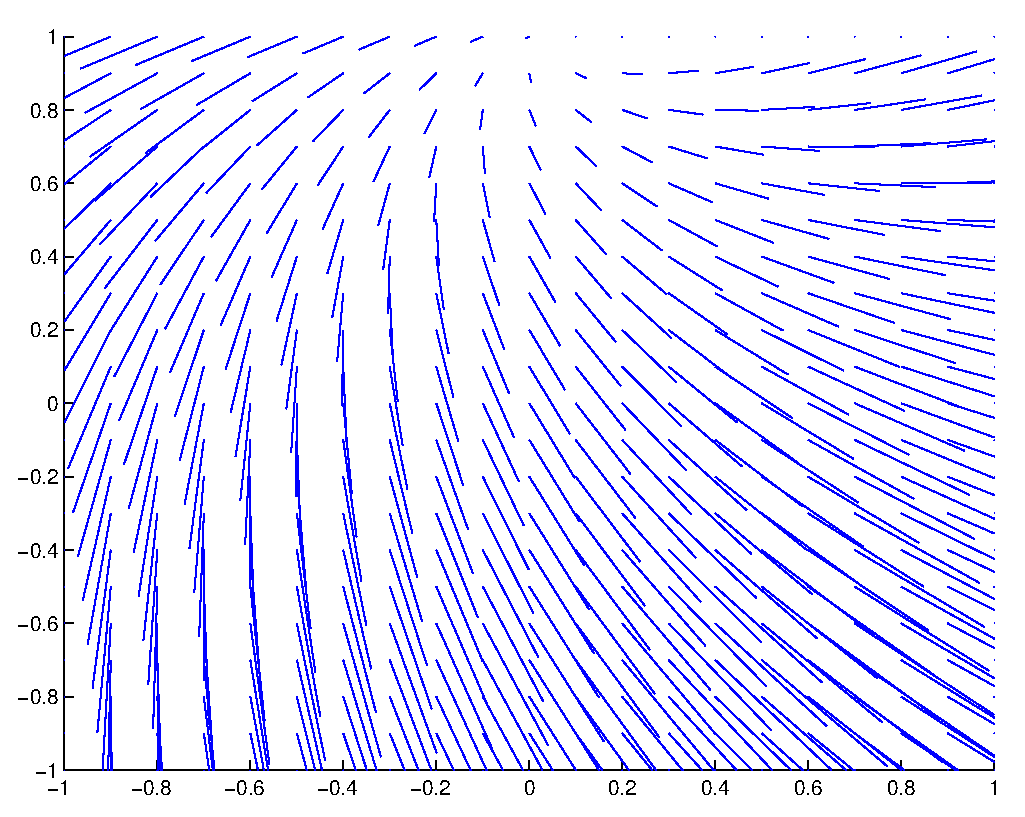
\includegraphics[width = 2in]{exampleFiles/stuff}
  \caption[Example small width figure]{
Example small width figure, showing how to use the width option.}
%
  \label{fig:intro_stuff2}
\end{figure}

\begin{figure}[t]
  \centering
  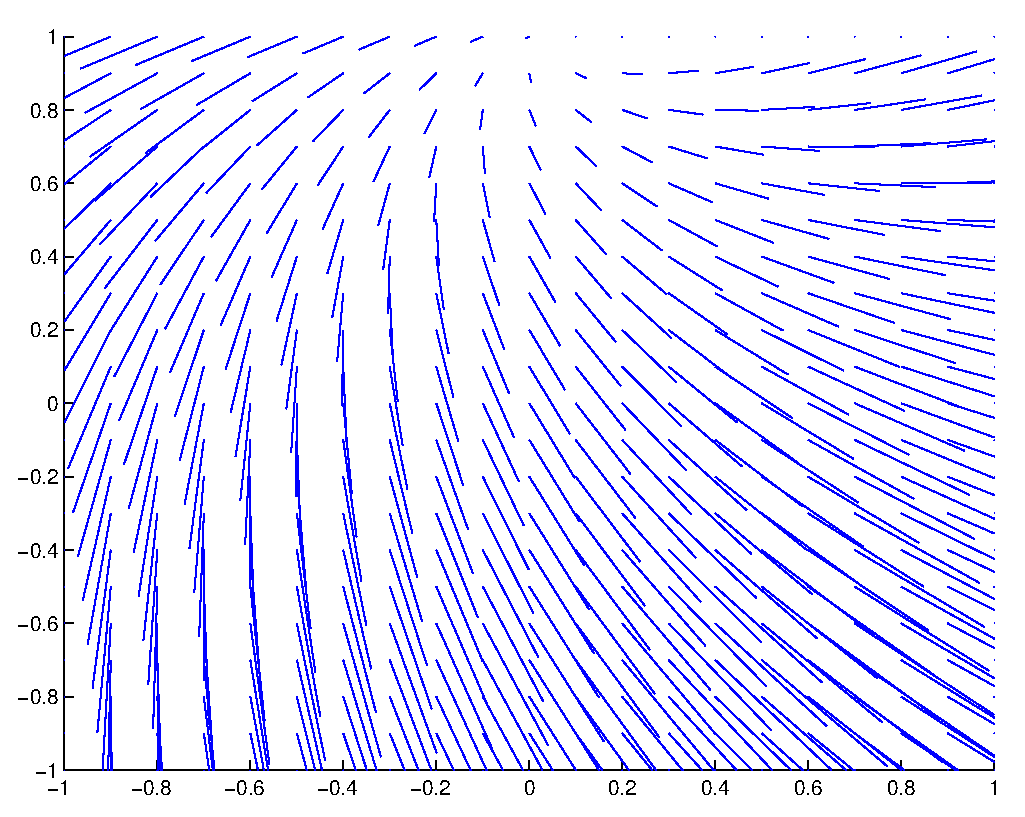
\includegraphics[width=5.5in]{exampleFiles/stuff}
  \caption[Example fixed width figure]{
This figure is just a simple figure with a width set at 5.5~in. An example of a
figure whose size depends on the width of the page is given in
Figure \ref{fig:appendix_some_pic} in Section~\ref{sec:appendixa_figure_example} of Appendix~\ref{apdx:appendixa}.}
%
  \label{fig:intro_stuff}
\end{figure}

%\begin{sidewaysfigure}[p]
%\includegraphics[scale=0.8]{examplegraphic}
%\caption{An example of a landscape graphic.}
%\label{fig:example}
%\end{sidewaysfigure}

\section{Math and Equation Example, Where the Heading Is Made so Long That It Extends onto a Second Line}
Here is how to use inline math mode to define lambda like this,
$\lambda$, and how to declare Equations~\eqref{eqn:definition_Ix}
and~\eqref{eqn:definition_Iy}

\begin{equation} \label{eqn:definition_Ix}
I_x(x,y) = \pd{I(x,y)}{x},
\end{equation}

\begin{equation}\label{eqn:definition_Iy}
I_y(x,y) = \pd{I(x,y)}{y}.
\end{equation}

 Or you can create equation arrays like
\begin{align}
  \alpha &= \beta^\gamma \\
  x &= \frac{1}{\alpha} \label{eq:cool_1} \\
  y &= \sqrt{\abs{\frac{\gamma}{\beta}}}  \\
  \zeta &= x^y \label{eq:cool_2}.
\end{align}


The lines in the array can be referenced by saying things like: In
Eqn.~\eqref{eq:cool_1} we show a wonderful equation, but it's not nearly as
amazing as Eqn.~\eqref{eq:cool_2}.
